% Visual system and reusable TikZ helpers.
\usepackage{lmodern}
\usepackage{fontspec}
\usefonttheme{professionalfonts}
\setsansfont{NimbusSans-Regular.otf}[Path=fonts/,BoldFont=NimbusSans-Bold.otf,ItalicFont=NimbusSans-Italic.otf,BoldItalicFont=NimbusSans-BoldItalic.otf]
\newfontfamily\editorial{P052-Italic.otf}[Path=fonts/]
\usepackage{amsmath,amssymb,graphicx,tikz}
\usetikzlibrary{arrows.meta,calc,shapes.geometric,decorations.pathreplacing}
\setbeamertemplate{navigation symbols}{}
\setbeamertemplate{headline}{}
\setbeamertemplate{footline}{}
\setbeamertemplate{frametitle}{}
\setbeamersize{text margin left=0pt,text margin right=0pt}
\definecolor{charcoal}{HTML}{17201D}
\definecolor{ivory}{HTML}{F4F0E7}
\definecolor{forest}{HTML}{245842}
\definecolor{gold}{HTML}{D9B45E}
\definecolor{goldink}{HTML}{88631D}
\definecolor{sage}{HTML}{A8C1AE}
\definecolor{muted}{HTML}{6B766D}
\definecolor{rulegray}{HTML}{D5D9CE}
\definecolor{softgreen}{HTML}{E4EADF}
\definecolor{softgold}{HTML}{EEE1BF}
\definecolor{stone}{HTML}{9DADA2}
\newcommand{\Dark}{\colorlet{bg}{charcoal}\colorlet{fg}{ivory}\colorlet{accent}{gold}\colorlet{subtle}{sage}\colorlet{linecol}{forest}}
\newcommand{\Light}{\colorlet{bg}{ivory}\colorlet{fg}{charcoal}\colorlet{accent}{forest}\colorlet{subtle}{muted}\colorlet{linecol}{rulegray}}
\newenvironment{canvas}{\begin{tikzpicture}[remember picture,overlay]\begin{scope}[shift={(current page.north west)},x=1cm,y=-1cm]\fill[bg] (0,0) rectangle (16,9);}{\end{scope}\end{tikzpicture}}
\hyphenpenalty=10000
\exhyphenpenalty=10000
\newcommand{\T}[6]{\pgfmathsetmacro{\leading}{#4*1.15}\node[anchor=north west,inner sep=0pt,align=left,text width=#3cm,text=#5,font=\fontsize{#4}{\leading}\selectfont] at (#1,#2) {#6};}
\newcommand{\C}[5]{\node[anchor=center,inner sep=0pt,text=#4,font=\fontsize{#3}{#3}\selectfont] at (#1,#2) {#5};}
\newcommand{\Header}[2]{\T{.8}{.52}{14}{7}{accent}{\textbf{#1}}\T{.8}{1.03}{14.4}{22}{fg}{\textbf{#2}}}
\newcommand{\Footer}[1]{\draw[linecol,line width=.35pt] (.8,8.39)--(15.2,8.39);\T{.8}{8.56}{12.9}{5.5}{subtle}{#1}\T{14.5}{8.52}{.7}{7}{subtle}{\textbf{\insertframenumber}\,/\,08}}
\newcommand{\Play}[3]{\fill[#3] (#1,#2) circle (.20);\fill[ivory] ({#1-.055},{#2-.09})--({#1-.055},{#2+.09})--({#1+.105},#2)--cycle;}
\newcommand{\Thumb}[5]{\begin{scope}\clip (#2,#3) rectangle ({#2+#4},{#3+#5});\node[anchor=north west,inner sep=0pt] at ({#2-(#1-1)*#4},{#3-(#4-#5)/2}) {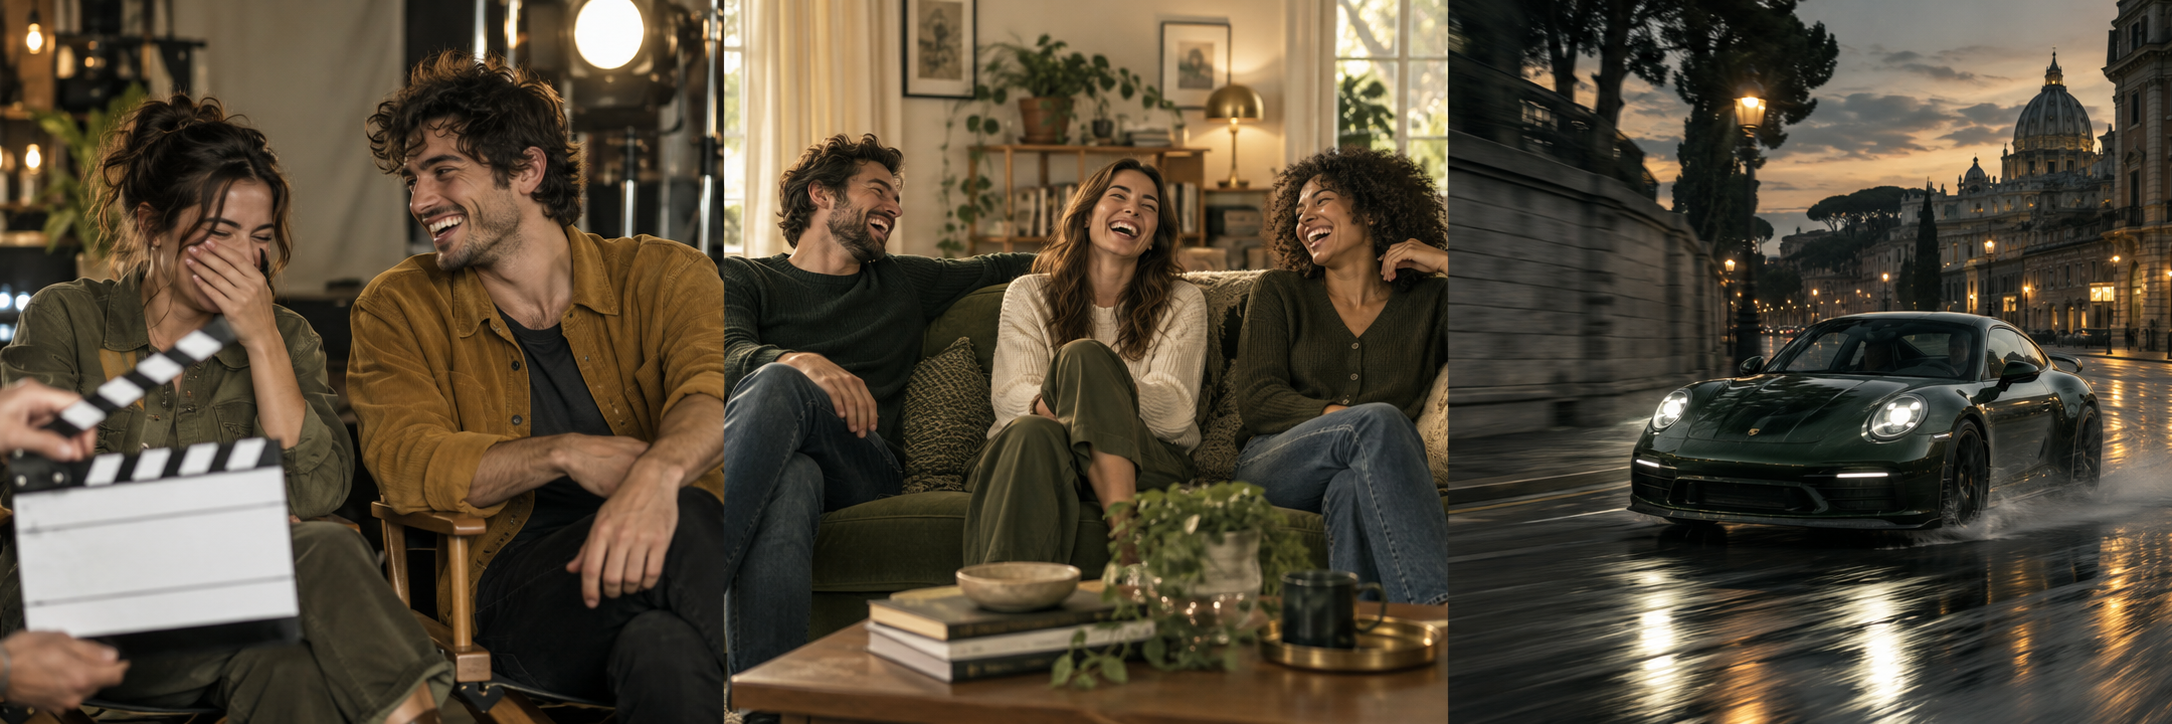
\includegraphics[width=\dimexpr#4cm*3\relax]{assets/videos.png}};\end{scope}}
\newcommand{\Force}[1]{\only<#1>{\relax}}
\title{Recommendation Algorithms: Bob's Next Video}
\author{Sami}
\date{}
\hypersetup{pdftitle={Recommendation Algorithms | Sami | Speaker 1},pdfauthor={Sami},pdfsubject={Feedback, user-item matrix, and content-based filtering},pdfpagemode=FullScreen}
